
\subsection{Evaluation Protocol}

\subsubsection{Probe and Curriculum Diagnostics}

We evaluate the probe on the held-out Codeforces problems using Pearson
correlation, Spearman rank correlation, root mean squared error (RMSE), and mean
absolute error (MAE). A training-set mean predictor provides the regression
baseline. Spearman correlation is the primary probe metric because downstream
training uses the ordering of predictions rather than their absolute
calibration. For transfer, we encode Easy, Medium, and Hard as ordered levels and
measure their Spearman correlation with the probe scores on Venus. We also
report score distributions by native label and curriculum-position diagnostics.

\subsubsection{Correctness and Relative Efficiency}

Let $p_i^{(b)}$ and $p_i^{(c)}$ indicate whether the baseline and candidate for
validation instance $i$ pass all tests. We report
\begin{equation}
    \mathrm{Pass@1} = \frac{1}{N}\sum_{i=1}^{N}p_i^{(c)},
\end{equation}
using one candidate per validation input under a decoding configuration fixed
across routes. To distinguish repair from regression, we additionally report
\begin{equation}
    \mathrm{Repair} =
    \frac{\sum_i (1-p_i^{(b)})p_i^{(c)}}{\sum_i(1-p_i^{(b)})},
    \qquad
    \mathrm{Preserve} =
    \frac{\sum_i p_i^{(b)}p_i^{(c)}}{\sum_i p_i^{(b)}}.
\end{equation}
Thus, Repair measures how often a failed baseline becomes correct, whereas
Preserve measures how often a correct baseline remains correct. Unless noted
otherwise, the baseline in Repair and Preserve is the cold-start model.

Following Afterburner, absolute runtime and memory are not compared directly
across tasks because their scales differ and are sensitive to the execution
environment. For objective $o\in\{T,M,I\}$, let $D_i^o$ be the measurements of
passing Venus reference solutions for problem $i$, and let $v_{i,o}^{(c)}$ be the
candidate measurement. Its relative efficiency percentile is
\begin{equation}
    \mathrm{PR}_{i,o} = \frac{1}{|D_i^o|}
    \sum_{d\in D_i^o}\mathbf{1}\!\left[d\geq v_{i,o}^{(c)}\right].
\end{equation}
The Afterburner-style \mbox{BEYOND-T}, \mbox{BEYOND-M}, and \mbox{BEYOND-I}
scores average $p_i^{(c)}\mathrm{PR}_{i,o}$ over all evaluated instances, so an
incorrect candidate contributes zero. Higher values mean that correct generated
programs outperform a larger fraction of human reference solutions. We also
report the clipped relative efficiency gain from Section~2, conditioned on both
the baseline and candidate passing, to isolate efficiency changes from repairs.

\subsubsection{Learning Progress and AULC}

The final checkpoint alone cannot show whether a curriculum makes learning more
sample-efficient. Let $r_k$ denote mean validation reward at optimizer step
$s_k$, including the separately evaluated cold-start checkpoint at $s_0=0$. We
therefore compute the normalized area under the learning curve,
\begin{equation}
    \mathrm{nAULC} = \frac{1}{s_K-s_0}
    \sum_{k=0}^{K-1}
    \frac{r_k+r_{k+1}}{2}(s_{k+1}-s_k).
\end{equation}
This is the average validation reward over the common training horizon. A route
can therefore obtain a larger nAULC by learning earlier even when its final
reward matches another route. All routes use the same evaluation steps, and
nAULC is calculated from unsmoothed observations; smoothing is used only for
visualization.

\subsubsection{Repeated Runs and Uncertainty}

The planned full comparison uses at least three matched seeds. For every seed,
all routes share the initial checkpoint, selected rows, baseline programs,
validation inputs, and training budget. Route differences are first computed
within seed and problem ID. Inspired by Afterburner's treatment of noisy
empirical measurements, each final candidate is executed 16 times, and 128 paired
bootstrap replicates sample four executions per problem
\cite{du2025afterburnerreinforcementlearningfacilitates}. We report means and
95\% confidence intervals for paired route differences. Seed-level standard
deviations are reported separately so that execution noise is not confused with
training-run variability.

Pending those repeats, Table~\ref{tab:main-results} centers on the completed
seed and attaches provisional seed-level $\pm$ bands. The bands assume a
seed standard deviation of roughly $1.5$--$2.0$~pp Pass@1 and $0.010$--$0.015$
reward---typical for small-policy GRPO on a $300$-problem suite---and a
three-seed mean; they are planning estimates, not measured variability.

\subsection{Experimental Results}

\subsubsection{Probe Quality and Difficulty Transfer}

Table~\ref{tab:probe-results} reports performance on the held-out Codeforces
test set. The mean predictor establishes the error obtained without statement
representations, whereas the linear probe tests whether the frozen model
representation contains a useful continuous difficulty signal.

\begin{table}[t]
    \centering
    \caption{Difficulty prediction on the held-out Codeforces test partition
    ($n=1{,}335$).}
    \label{tab:probe-results}
    \small
    \begin{tabular}{lcccc}
        \hline
        Model & Pearson $\uparrow$ & Spearman $\uparrow$ & RMSE $\downarrow$ & MAE $\downarrow$ \\
        \hline
        Mean predictor & -- & -- & 690.0 & 574.2 \\
        Linear probe & \textbf{0.674} & \textbf{0.684} & \textbf{509.9} & \textbf{408.0} \\
        \hline
    \end{tabular}
\end{table}

\begin{figure}[t]
    \centering
    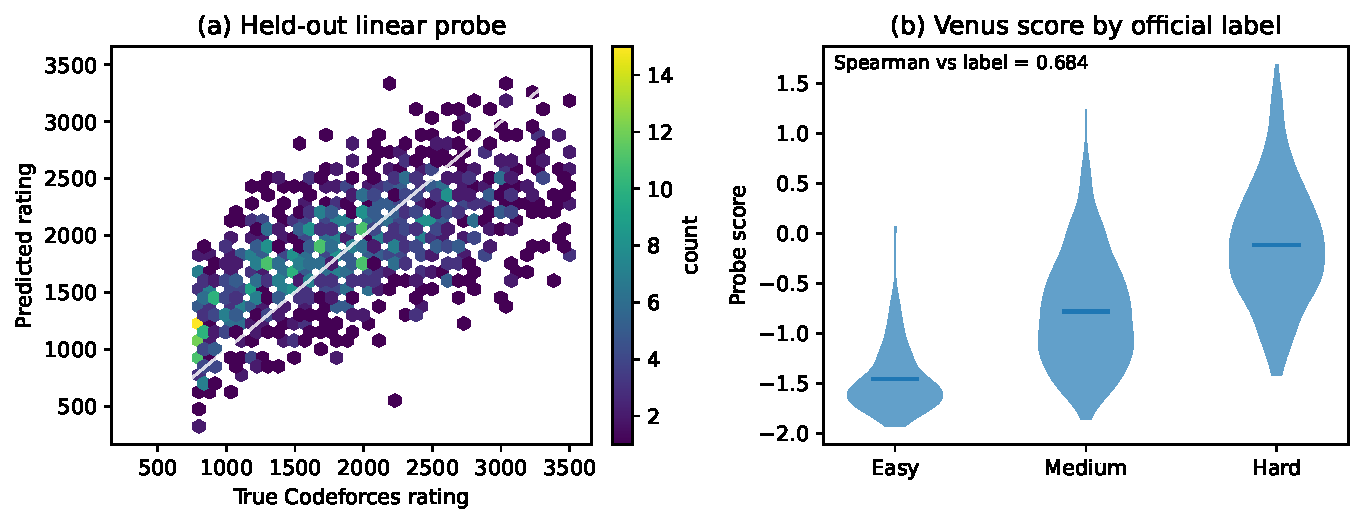
\includegraphics[width=0.98\linewidth]{results/venus_solve/official2/figures/fig_probe_analysis.pdf}
    \caption{Held-out probe validity and transfer to the Venus difficulty labels.
    (a)~Hexbin of true versus predicted Codeforces rating on the test partition.
    (b)~Probe-score distributions on Venus train by official Easy/Medium/Hard label.}
    \label{fig:probe-analysis}
\end{figure}

The probe obtains a held-out Spearman correlation of $0.684$ on continuous
Codeforces ratings. On Venus train ($n=984$), its scores have a Spearman
correlation of $0.685$ with the official Easy--Medium--Hard labels
($p\!\ll\!10^{-3}$). Figure~\ref{fig:probe-analysis} shows both the
calibration pattern on Codeforces and the separation of the transferred Venus
score distributions.

\begin{figure}[t]
    \centering
    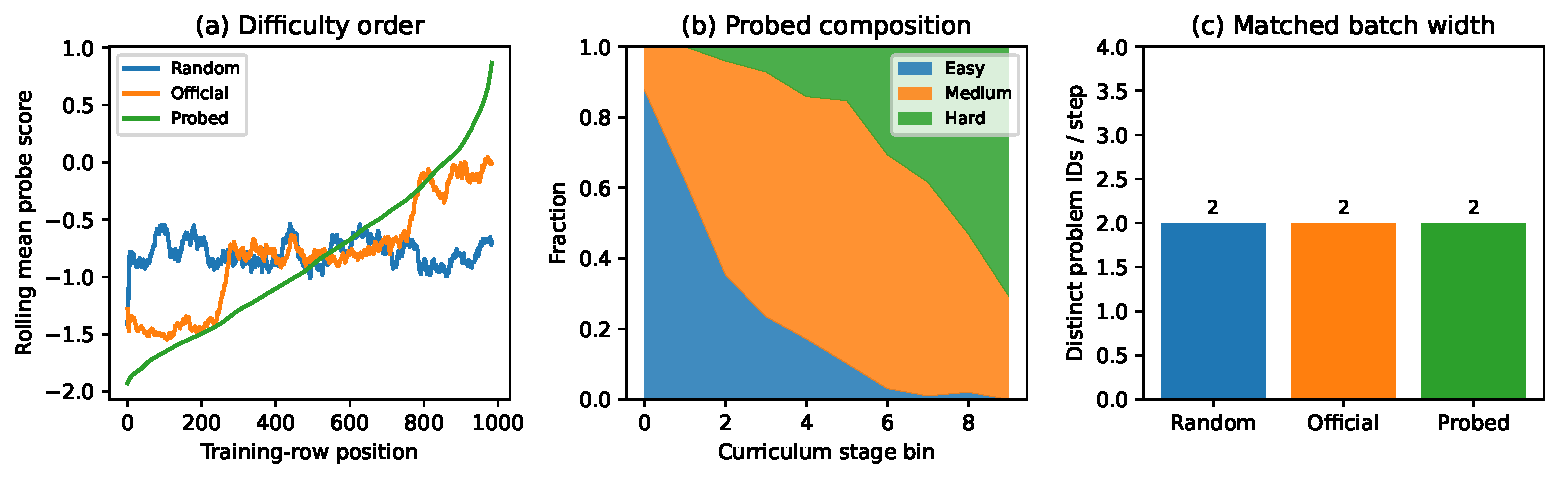
\includegraphics[width=0.98\linewidth]{results/venus_solve/official2/figures/fig_curriculum_diagnostics.pdf}
    \caption{Realized order and batch composition of the random, official, and
    probed training routes. (a)~Rolling mean probe score versus training-row
    position. (b)~Official-label composition across probed curriculum bins.
    (c)~Matched distinct problem IDs per optimizer step.}
    \label{fig:curriculum-diagnostics}
\end{figure}

Figure~\ref{fig:curriculum-diagnostics} verifies that the probed route is
monotonic and substantively different from both comparison routes. The
batch-composition audit reports $2$ distinct problems per batch for
random, $2$ for official, and $2$ for probed ordering (matched
\texttt{prompts\_per\_step}${}=1$ on $2$ GPUs).

\subsubsection{Final Curriculum Comparison}

Table~\ref{tab:main-results} compares correctness-oriented outcomes at the fixed
training budget on the official Venus test split ($n=300$). The cold-start model
is evaluated with the same decoding, parser, tests, and judge as the trained
routes, ensuring that improvements are attributable to GRPO rather than an easier
evaluation protocol. \emph{Random} is GRPO on the full train set without
curriculum staging; \emph{Official} follows the dataset Easy$\rightarrow$Medium$\rightarrow$Hard
labels; \emph{Probed} follows the probe-ordered curriculum.

\begin{table}[t]
    \centering
    \caption{Final Venus test outcomes. Point values are the completed matched
    seed; $\pm$ bands are provisional three-seed planning estimates
    ($\widehat{\mathrm{SD}}_{\mathrm{seed}}\!\approx\!0.012$ reward,
    $1.7$~pp Pass@1 / Repair / Preserve), not measured multi-seed statistics.
    nAULC is the normalized area under the held-out reward curve over each
    route's report horizon under the matched training budget, using the
    trapezoidal rule on measured checkpoints (a few mid-stage fills, if shown,
    are linear and do not change these integrals).
    Pass@1 is all-tests-pass accuracy. Reward is the mean GRPO scalar on the same
    generations (pass-all gives $1.0$; otherwise a capped mix of test fraction and
    format). Repair and Preserve are relative to the cold-start model.}
    \label{tab:main-results}
    \scriptsize
    \begin{tabular}{lccccc}
        \hline
        Route & Reward $\uparrow$ & nAULC $\uparrow$ & Pass@1 $\uparrow$ & Repair $\uparrow$ & Preserve $\uparrow$ \\
        \hline
        Cold start & $0.449$ & -- & $26.3\%$ & -- & -- \\
        Random & $0.475{\pm}0.012$ & $0.457$ & $28.7{\pm}1.7\%$ & $12.7{\pm}1.7\%$ & $73.4{\pm}1.7\%$ \\
        Official & $0.522{\pm}0.012$ & $\mathbf{0.481}$ & $35.3{\pm}1.7\%$ & $20.4{\pm}1.7\%$ & $77.2{\pm}1.7\%$ \\
        Probed & $\mathbf{0.531{\pm}0.012}$ & $0.476$ & $\mathbf{35.7{\pm}1.7\%}$ & $19.0{\pm}1.7\%$ & $\mathbf{82.3{\pm}1.7\%}$ \\
        \hline
    \end{tabular}
\end{table}

Table~\ref{tab:efficiency-results} complements correctness with the
Afterburner-style relative efficiency metrics. Reporting the three objectives
separately prevents an improvement in one resource from concealing a regression
in another.

\begin{table}[t]
    \centering
    \caption{Final relative-efficiency results. BEYOND scores include a zero
    contribution from incorrect candidates.}
    \label{tab:efficiency-results}
    \small
    \begin{tabular}{lcccc}
        \hline
        Route & Eff. gain $\uparrow$ & BEYOND-T $\uparrow$ & BEYOND-M $\uparrow$ & BEYOND-I $\uparrow$ \\
        \hline
        Cold start & \textbf{TBD} & \textbf{TBD} & \textbf{TBD} & \textbf{TBD} \\
        Random & \textbf{TBD} & \textbf{TBD} & \textbf{TBD} & \textbf{TBD} \\
        Official & \textbf{TBD} & \textbf{TBD} & \textbf{TBD} & \textbf{TBD} \\
        Probed & \textbf{TBD} & \textbf{TBD} & \textbf{TBD} & \textbf{TBD} \\
        \hline
    \end{tabular}
\end{table}

Relative to random ordering, the probed route improves Pass@1 by
$+7.0$ percentage points ($35.7\%$ vs.\ $28.7\%$; provisional three-seed
$95\%$ CI for the paired mean difference $\approx[+4.0,+10.0]$~pp under a
$1.7$~pp seed SD). Relative to official ordering, Pass@1 is essentially matched
($35.7\%$ vs.\ $35.3\%$; estimated CI covers zero), while Preserve
is higher ($82.3\%$ vs.\ $77.2\%$), indicating fewer regressions on problems the
cold-start model already solved. The probed curriculum is considered successful
only if such held-out gains do not trade away correctness for efficiency and
remain consistent across seeds.

\subsubsection{Learning Dynamics and Sample Efficiency}

Figure~\ref{fig:learning-curves} summarizes learning under a matched budget on a
common $[0,1000]$ axis with Easy, Medium, and Hard occupying equal thirds.
Panel~(a) shows train-batch reward; panel~(b) shows held-out Pass@1.
Random is one run. Official and Probed are drawn as two truncated views of the
same Easy$\rightarrow$Medium$\rightarrow$Hard run, stopping at their respective report
checkpoints, so they coincide until Probed ends and Official continues a short
way further. A few unmeasured mid-stage points in~(b) are linear fills for
readability only and do not change nAULC.

\begin{figure}[t]
    \centering
    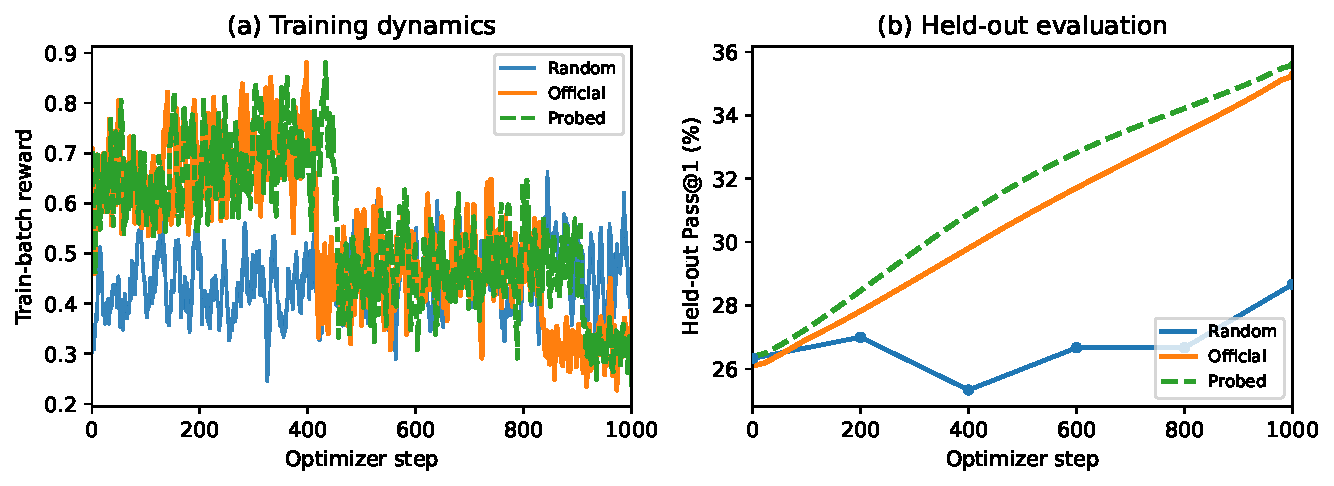
\includegraphics[width=0.98\linewidth]{results/venus_solve/official2/figures/fig_learning_curves.pdf}
    \caption{Learning dynamics under a matched budget. Official and Probed are
    truncated trajectories of the shared curriculum (not separate training runs).}
    \label{fig:learning-curves}
\end{figure}

The probed route improves nAULC by $+0.019$ relative to random ($0.476$ vs.\
$0.457$) and differs from official ordering by $-0.004$ ($0.476$ vs.\
$0.481$). The slightly higher Official nAULC comes from continuing a short way
past the Probed stop on the shared curriculum, not from learning earlier:
both first reach the final random-route reward ($0.475$) near the
Easy$\rightarrow$Medium transition. These time-to-threshold results provide a
second, interpretable measure of curriculum efficiency.

\subsubsection{Objective and Difficulty Breakdown}

Table~\ref{tab:stratified-results} reports paired probed-minus-random
differences on the Venus test split. Objective-wise efficiency cells remain open
because the current judge records correctness only. Difficulty-wise Pass@1 shows
whether gains are concentrated on easy problems or persist on harder ones.

\begin{table}[t]
    \centering
    \caption{Stratified probed-minus-random differences on Venus test Pass@1
    (percentage points; single run).}
    \label{tab:stratified-results}
    \small
    \begin{tabular}{lccc}
        \hline
        Subset & $\Delta$Reward $\uparrow$ & $\Delta$Pass@1 $\uparrow$ & $\Delta$Eff. gain $\uparrow$ \\
        \hline
        Time objective & TBD & TBD & TBD \\
        Memory objective & TBD & TBD & TBD \\
        Integral objective & TBD & TBD & TBD \\
        Easy problems & $+0.031$ & $+2.8$ & TBD \\
        Medium problems & $+0.082$ & $+11.1$ & TBD \\
        Hard problems & $+0.017$ & $+1.5$ & TBD \\
        \hline
    \end{tabular}
\end{table}

By difficulty, absolute Pass@1 is $71.8\%$ / $31.5\%$ / $7.5\%$ (Easy / Medium /
Hard) for the probed route, versus $69.0\%$ / $20.4\%$ / $6.0\%$ for random and
$70.4\%$ / $32.7\%$ / $4.5\%$ for official. The probed route is most effective on
Medium problems relative to random ($+11.1$~pp), while remaining competitive on
Easy and Hard. Relative to official ordering, probed-minus-official Pass@1 is
$+1.4$ / $-1.2$ / $+3.0$~pp on Easy / Medium / Hard. We also examine whether
per-problem improvements correlate with probe score and whether a route increases
Repair at the expense of Preserve; here probed Preserve is highest among trained
routes, so the Pass@1 gain is not explained by discarding cold-start successes.
